\section{Декартово дерево}
Декартово дерево: построение декартова дерева за линейное время
(при предварительно отсортированных ключах),
реализация операций вставки и удаления через split и merge.
Treap: верхняя оценка $\O(\log n)$ на мат. ожидание
глубины конкретной вершины, глубины средней вершины,
глубины дерева.
Использование неявного ключа, rope.

\subsection{Декартово дерево}
Декартово дерево --- двоичное дерево поиска по ключу
и одновременно куча по приоритету.

Декартово дерево существует и единственно
для любого набора различных ключей и приоритетов,
доказательство --- алгоритм построения за квадрат
(взять в наборе максимальный приоритет,
это будет корень дерева,
все ключи меньше него слева,
все ключи больше него справа,
повторить рекурсивно для обоих поддеревьев).

При предварительно отсортированных ключах
можно построить за линейное время:
проходим по вершинам слева направо,
имеем 3 случая
(ось абсцисс --- ключ, ось ординат --- приоритет):

\bigskip

\noindent
\begin{minipage}{\textwidth}
    \begin{center}
        Вершина добавляется к существующей самой правой:

        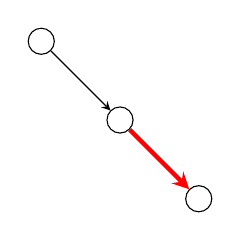
\begin{tikzpicture}[
            every node/.style={draw,circle},
            every path/.style={->,>=stealth}
            ]
            \node (x1) at (1, 3) {};
            \node (x2) at (2, 2) {};
            \node (x3) at (3, 1) {};
            \draw[->] (x1) -- (x2);
            \draw[->,ultra thick,red] (x2) -- (x3);
        \end{tikzpicture}
    \end{center}
\end{minipage}

\bigskip

\noindent
\begin{minipage}{\textwidth}
    \begin{center}
        Вершина становится новым корнем:

        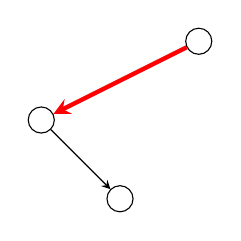
\begin{tikzpicture}[
            every node/.style={draw,circle},
            every path/.style={->,>=stealth}
            ]
            \node (x1) at (1, 2) {};
            \node (x2) at (2, 1) {};
            \node (x3) at (3, 3) {};
            \draw (x1) -- (x2);
            \draw[ultra thick,red] (x3) -- (x1);
        \end{tikzpicture}
    \end{center}
\end{minipage}

\bigskip

\noindent
\begin{minipage}{\textwidth}
    \begin{center}
        Часть дерева переподвешивается к вершине:

        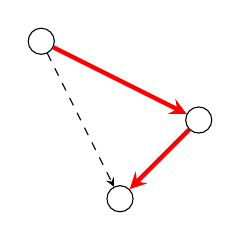
\begin{tikzpicture}[
            every node/.style={draw,circle},
            every path/.style={->,>=stealth}
            ]
            \node (x1) at (1, 3) {};
            \node (x2) at (2, 1) {};
            \node (x3) at (3, 2) {};
            \draw[dashed] (x1) -- (x2);
            \draw[ultra thick,red] (x3) -- (x2);
            \draw[ultra thick,red] (x1) -- (x3);
        \end{tikzpicture}
    \end{center}
\end{minipage}

\bigskip

Можно заметить, что проход наверх по каждому ребру
произойдёт не более одного раза, а количество
всех рёбер --- $n - 1$.
Поэтому мы идём слева направо по ключам,
и время построения декартова дерева --- $\O(n)$.

Операции split и merge:

\noindent
\begin{minipage}{\textwidth}
    \begin{algorithmic}
        \Function{split}{$T, v$}
            \LComment{Всё примерно очевидно}
            \If{$T = \None$}
                \Return $\langle \None; \None \rangle$
            \EndIf
            \State $x$ --- ключ в корне
            \State $p$ --- приоритет в корне
            \State $L$ --- левое поддерево
            \State $R$ --- правое поддерево
            \If{$x < v$}
                \State $\langle T_l; T_r \rangle \gets \Call{split}{R, x}$
                \State $T_n \gets \Call{node}{x, p, L, T_l}$
                \State \Return $\langle T_n; T_r \rangle$
            \Else
                \State $\langle T_l; T_r \rangle \gets \Call{split}{L, x}$
                \State $T_n \gets \Call{node}{x, p, T_r, R}$
                \State \Return $\langle T_l; T_n \rangle$
            \EndIf
        \EndFunction
    \end{algorithmic}
\end{minipage}

\bigskip

\noindent
\begin{minipage}{\textwidth}
    \begin{algorithmic}
        \Function{merge}{$T_1, T_2$}
            \Comment{$\forall x \in T_1.~\forall y \in T_2.~x \le y$}
            \If{$T_1 = \None$}
                \Return $T_2$
            \EndIf
            \If{$T_2 = \None$}
                \Return $T_1$
            \EndIf
            \State $x_1$ --- значение в корне первого поддерева
            \State $x_2$ --- значение в корне второго поддерева
            \State $p_1$ --- приоритет корня первого поддерева
            \State $p_2$ --- приоритет корня второго поддерева
            \State $L_1$ --- левое поддерево первого поддерева
            \State $L_2$ --- левое поддерево второго поддерева
            \State $R_1$ --- правое поддерево первого поддерева
            \State $R_2$ --- правое поддерево второго поддерева
            \If{$p_1 < p_2$}
                \State $T_n \gets \Call{merge}{T_1, L_2}$
                \State \Return $\Call{node}{x_2, p_2, T_n, R_2}$
            \Else
                \State $T_n \gets \Call{merge}{T_2, R_1}$
                \State \Return $\Call{node}{x_1, p_1, L_1, T_n}$
            \EndIf
        \EndFunction
    \end{algorithmic}
\end{minipage}

Тогда добавление и удаление очевидно реализуются
через split и merge.

\begin{definition}
    Дуча, treap, курево, дерамида --- декартово дерево,
    построенное на независимых случайных приоритетах.
\end{definition}

\begin{theorem}
    Математическое ожидание высоты дерамиды --- $\O(\log n)$.
\end{theorem}
\begin{proof}
    Существует однозначное соответствие между дерамидами
    и деревьями быстрой сортировки.
    Считая оценку для глубины рекурсии быстрой сортировки доказанной,
    получаем оценку для глубины дерамиды.
\end{proof}

Декартово дерево по неявному ключу:
храним количество вершин в левом поддереве,
ключ --- количество вершин, предшествующих данной,
считаем его для вершины по мере спуска к ней.
Очевидно, все свойства выполняются.
